\chapter{Indledning}

\chapter{Kravspecifikation}
\section{Godkendelsesformular}
\begin{table}[h!]
\label{tab:tabel2}
\begin{tabular}{| l | >{\raggedright\arraybackslash}p{12cm} |}
   \hline
   \textbf{Forfattere} & Ida, Line, Mette, Brian, Mohamed og Khaled\\ \hline
   \textbf{Godkendes af:} & Samuel Alberg Thrysøe\\ \hline
   \textbf{Antal sider:} & \\ \hline
   \textbf{Kunde:} & IHA\\ \hline
\end{tabular}
\end{table}
\textbf{Ved underskrivelse af dette dokument accepteres det af begge parter, som værende kravene til udviklingen af det ønskede system.}
\newline
\textbf{Sted og dato:}\\
\\
\\
\begin{table}
[h!]
\begin{tabular}{ l lllllllll l}
--------------------------------------&&&&&&&&&&--------------------------------------\\ 
Kundens underskrift &&&&&&&&&&Leverandørens underskrift\\
\end{tabular}
\end{table}
\section{Indledning}
Denne kravspecifikation er blevet udarbejdet på baggrund af krav fra kunden, samt hvad leverandøren finder muligt. Kravspecifikationens formål er at specificere de krav, der er til produktet. 
\newpage

\section{Systembeskrivelse}
Blodtryksmålersystemet ønskes at kunne måle blodtryk, EKG og iltmætning for en patient. Ud fra blodtrykket findes systolisk, diastolisk og middeltryks værdier, dette gøres ved at finde den maksimale værdi (systole) og den minimale værdi (diastole) for blodtrykskurven. Ud fra disse to værdier bestemmes middeltrykket, dette gøres ved formlen: $middel = 1/3 \cdot systole + 2/3 \cdot diastole$. Ud fra EKG-signalet kan pulsen bestemmes, dette gøres ved at bestemme antallet af R-takker på et minut. Desuden kan pulsen bestemmes ud fra blodtrykket, da pulsen her er antallet af systoliske værdier på et minut. Iltmætningen er mængden af ilt i blodet. For at kunne bestemme denne værdi skal et eksternt produkt benyttes. Dette produkt skal ved hjælp at infrarød bestemme iltmætningen i blodet. 
\newpage

\section{Aktør-kontekst diagram}
\begin{figure}[h!]
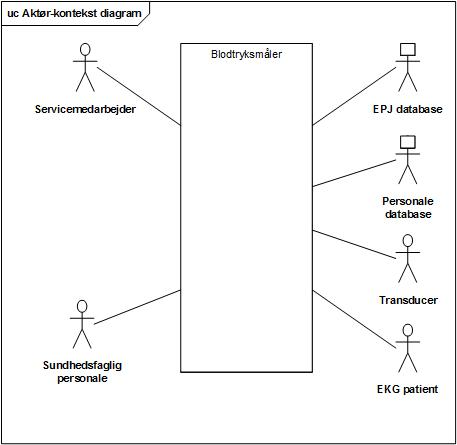
\includegraphics[width =0.65\textwidth , center]{billeder/Aktorkontekst.jpg}
\caption{\textbf{Aktør-kontekst diagram}}
\end{figure}

Af dette diagram ses de interagerende aktører: \textit{Sundhedsfaglig personale}, \textit{Transducer}, \textit{EKG patient}, \textit{EPJ database}, \textit{Personale database} og \textit{Servicemedarbejder}.\\ Herunder er der en detaljeret beskrivelse af hver aktør.

\begin{table}[h!]
\begin{tabular}{| >{\raggedright\arraybackslash}p{3cm} | >{\raggedright\arraybackslash}p{12cm} |}
   \hline
   Navn: & Sundhedsfaglig personale\\ \hline
   Type: & Primær aktør \\ \hline
   Beskrivelse: & Det sundhedsfaglige personale er aktøren, der sætter måleudstyret til transduceren, samt starter målingen. Det er det sundhedsfaglige personale, der interagerer med systemet og dermed har tilgang til de viste målinger på brugergrænsefladerne (startskærm og hovedskærm).\\ \hline
\end{tabular}
\end{table}


\begin{table}[h!]
\begin{tabular}{| >{\raggedright\arraybackslash}p{3cm} | >{\raggedright\arraybackslash}p{12cm} |}
   \hline
   Navn: & Transducer\\ \hline
   Type: & Sekundær aktør \\ \hline
   Beskrivelse: & Transduceren er kilden til måleresultaterne, og dermed fungerer som patienten. I dette tilfælde er det en vandsøjle der leverer et tryk i mmHg. Måleresultater opnås ved, at disse data sendes ind i systemet igennem hardwaren.\\ \hline
\end{tabular}
\end{table}

\begin{table}[h!]
\begin{tabular}{| >{\raggedright\arraybackslash}p{3cm} | >{\raggedright\arraybackslash}p{12cm} |}
   \hline
   Navn: & EKG patient\\ \hline
   Type: & Sekundær aktør \\ \hline
   Beskrivelse: & EKG patienten er den aktør hvorfra værdierne til EKG-kurven fås fra. Dermed er det denne aktør der er kilden til pulsen. Disse værdier hentes fra PhysioBank ATM.\\ \hline
\end{tabular}
\end{table}


\begin{table}[h!]
\begin{tabular}{| >{\raggedright\arraybackslash}p{3cm} | >{\raggedright\arraybackslash}p{12cm} |}
   \hline
   Navn: & Personale database\\ \hline
   Type: & Sekundær aktør \\ \hline
   Beskrivelse: & Personale database er der, hvori det sundhedsfaglige personales login informationer opbevares, hvilket benyttes til at tilgå systemet. \\ \hline
\end{tabular}
\end{table}


\begin{table}[h!]
\begin{tabular}{| >{\raggedright\arraybackslash}p{3cm} | >{\raggedright\arraybackslash}p{12cm} |}
   \hline
   Navn: & EPJ database\\ \hline
   Type: & Sekundær aktør \\ \hline
   Beskrivelse: & EPJ database er den database, hvor patientdata ligger, samt der hvori analyseresultaterne, der opnås ved målingerne i systemet, samt signalerne bliver gemt. Disse data er grafer for EKG, arterietryk, samt talværdier for puls, systole, diastole og middeltryk. Denne EPJ database skal simulere den EPJ database der fungere på sygehusene i virkeligheden.\\ \hline
\end{tabular}
\end{table}


\begin{table}[h!]
\begin{tabular}{| >{\raggedright\arraybackslash}p{3cm} | >{\raggedright\arraybackslash}p{12cm} |}
   \hline
   Navn: & Servicemedarbejder\\ \hline
   Type: & Primær aktør \\ \hline
   Beskrivelse: & Servicemedarbejderen er aktøreren der igangsætter og foretager kalibreringen.\\ \hline
\end{tabular}
\end{table}

\newpage

\section{Use cases}
\begin{figure}[H]
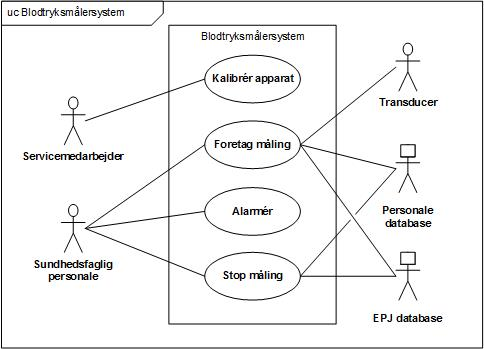
\includegraphics[width =0.7\textwidth , center]{billeder/UseCaseDiagram}
\caption{\textbf{Use case diagram}}
\end{figure}

De fire Use cases kan ses ud fra Use case diagrammet, disse er: \textit{Kalibrér apparat}, \textit{Foretag måling}, \textit{Alarmér} og \textit{Stop måling}. Hver enkel af disse Use cases beskrives detaljeret herunder i et fully-dressed Use case skema.\\
Systemet består af en computer med programkode, en NI-DAQ samt hardware. Hardwaren består af et lavpasfilter, en forstærker og en transducer desuden er der hertil tilkoblet to 9 V batterier.
\\
Systemet gør det muligt at hente data fra transduceren. Her går data fra transduceren igennem forstærkeren, hvilken bliver forsynet af spænding fra to 9 V batterier. Fra forstærkeren går signalet videre til lavpasfilteret og derefter ind i NI-DAQ, som så sender data videre til computeren og ind i programkoden. 
\\ 

"Signalets vej" og opbygning beskrives\\\\

Det digitale filter er pr. default slået til når systemet startes, dog vil det være muligt at slå dette filter fra under målingen.\\
Når programmet startes skal computeren have VPN-forbindelse til "ASE IHA VPN", desuden skal der være en forbindelse til $"webhotel10.F15ST2ITS2201404669.db_{-}owner"$, da det er herunder de to databaser; Personale database og EPJ database ligger.\\\\
Programmet skal have to skærme; en startskærm, der fungerer som EPJ systemet, og en hovedskærm, der fungerer som selve blodtryksmålerens grænseflade.

\begin{table}[H]
\caption{Use case 1}\label{tab:tabel3}
\begin{tabular}{| l | >{\raggedright\arraybackslash}p{11cm} |}
   \hline
   \textbf{Use case 1} & \textbf{Kalibrér apparat}\\ \hline
   Mål: & Få kalibreret apparatet \\ \hline
   Initiering: & Startes af Servicemedarbejder\\ \hline
   Aktører:& Servicemedarbejder (primær)\\ \hline
   Referencer: & - \\ \hline
   Samtidige forekomster: & én kalibrering pr. apparat \\\hline
   Forudsætninger: & Blodtryksmålersystemet er tændt og tilsluttet kalibreringsudstyret.\\ \hline
   Resultat:& Apparatet er kalibreret\\ \hline
   Hovedscenarie:& 
1. Servicemedarbejder foretager kalibreringen, ved at indtaste spændingen og trykket for de tre målepunkter fra væskesøjlen.\newline
2. Systemet beregner kalibreringsværdien.\\\hline
Udvidelse/undtagelser: & - \\\hline
\end{tabular}
\end{table}


\begin{table}[H]
\caption{Use case 2}\label{tab:tabel3}
\begin{tabular}{| l | >{\raggedright\arraybackslash}p{11cm} |}
   \hline
   \textbf{Use case 2} & \textbf{Foretag måling}\\ \hline
   Mål: & Den valgte patients målinger foretages og værdierne gemmes i EPJ database\\ \hline
   Initiering: & Startes af Sundhedsfaglig personale\\ \hline
   Aktører:& Sundhedsfaglig personale (primær), Personale database (sekundær), EPJ database(sekundær), Transducer (sekundær), EKG patient (sekundær)\\ \hline
   Referencer: & Use case 2 \\ \hline
   Samtidige forekomster: & Én sundhedsfaglig person og én transducer pr. system \\\hline
   Forudsætninger: & VPN, Personale database og EPJ databasen er tilsluttet korrekt\\ \hline
   Resultat:& Målingerne for den valgte patient er foretaget\\ \hline
   Hovedscenarie:& 
1. Sundhedsfaglig personale logger på ved at indtaste brugernavn og kode. \newline
   \textit{$[$Undtagelse 1: Brugernavn og/eller kode indtastet forkert$]$}\newline
2. Besked: "Logget på" vises  \newline
3. Liste med patienter kommer frem\newline
4. Den ønskede patient vælges \newline
5. Sundhedsfaglig personale starter målingen \newline
6. Systemet indhenter data fra transduceren og måler, hvor lang tid målingen foretages\newline
7. EKG og arterietryk præsenteres kontinuert på hver sin graf. Puls, systole, diastole og middeltryk vises som talværdier. Data gemmes automatisk kontinuert i EPJ database. \newline
\textit{$[$Udvidelse 1: Slå digitalt filter til/fra$]$}\newline
\textit{$[$Udvidelse 2: Juster systolens/diastolens grænseværdi$]$}\newline
8. Sundhedsfaglig personale trykker på "Nulpunks justering"\newline
9. Systemet starter nulpunkts justeringen. \\\hline
Udvidelse/undtagelser: & $[$Undtagelse 1: Brugernavn og/eller kode indtastet forkert$]$\newline
1.1 Besked: "Brugernavn og/eller kode indtastet forkert"\newline
1.2 Use case 3 starter forfra \newline\newline
$[$Udvidelse 1: Slå digitalt filter til/fra$]$\newline 
1.1 Sundhedsfaglig personale vælger "Digitalt filter OFF" \newline
1.2 Systemet slår det digitale filter fra\newline
1.3 Sundhedsfaglig personale vælger "Digitalt filter ON"\newline
1.4 Systemet slår det digitale filter til\newline\newline
$[$Udvidelse 2: Juster systolens/diastolens grænseværdi$]$\newline
2.1 Sundhedsfaglig personale justerer grænseværdierne for systole og/eller diastole.
\\\hline
\end{tabular}
\end{table}


\begin{table}[H]
\caption{Use case 3}\label{tab:tabel3}
\begin{tabular}{| l | >{\raggedright\arraybackslash}p{11cm} |}
   \hline
   \textbf{Use case 3} & \textbf{Alarmér}\\ \hline
   Mål: & Få startet alarmeringen ved overskridelse af en grænseværdi \\ \hline
   Initiering: & Systemet starter denne Use case\\ \hline
   Aktører:& Sundhedsfaglig personale (sekundær)\\ \hline
   Referencer: & Use case 2 \\ \hline
   Samtidige forekomster: & - \\\hline
   Forudsætninger: & Målingen i Use case 2: Foretag måling, er kørt succesfuldt \\ \hline
   Resultat:& Alarmen starter\\ \hline
   Hovedscenarie:& 
1. Grænseværdi overskrides \newline
2. Alarm starter med lyd og tallet, hvis grænseværdi er overskredet skifter farve til hvid.\newline
    \textit{$[$Udvidelse 1: Anden grænseværdi overskrides$]$} \newline
    \textit{$[$Udvidelse 2: Udsæt alarm$]$ }\newline
3. Alarmen stopper når grænseværdien ikke længere er overskredet.
\\\hline
Udvidelse/undtagelser: & $[$Udvidelse 1: Anden grænseværdi overskrides$]$ \newline
1.1. Endnu en grænseværdi overskrides\newline
1.2. Lyden fra første alarm fortsætter. Det nye tal som har overskredet grænseværdien skifter ligeledes farve til hvid.\newline
1.3 Use case afsluttet.\newline\newline
$[$Udvidelse 2: Udsæt alarm$]$\newline
2.1 Sundhedsfaglig person udsætter alarm\newline
2.2 Systemet stopper alarmens lyd i et minut
\\\hline
\end{tabular}
\end{table}


\begin{table}[H]
\caption{Use case 4}\label{tab:tabel3}
\begin{tabular}{| l | >{\raggedright\arraybackslash}p{11cm} |}
   \hline
   \textbf{Use case 4} & \textbf{Stop måling}\\ \hline
   Mål: &  Få stoppet målingen og logget ud\\ \hline
   Initiering: & Startes af Sundhedsfaglig personale \\ \hline
   Aktører: & Sundhedsfaglig personale (primær) \\ \hline
   Referencer: & Use case 2\\ \hline
   Samtidige forekomster: & - \\\hline
   Forudsætninger: & Use case 2: Foretag måling, er kørt succesfuldt\\ \hline
   Resultat:& Signalet er stoppet, sundhedsfaglig personale er logget ud og vendt tilbage til startskærm.\\ \hline
   Hovedscenarie:& 
1. Sundhedsfaglig personale stopper måling\newline
2. Systemet stopper målingen.\newline 
3. Sundhedsfaglig personale logger ud \\\hline
Udvidelse/undtagelser: & -\\\hline
\end{tabular}
\end{table}



\newpage 
\newpage 
\newpage
\newpage



\section{Ikke-funktionelle krav}
De ikke-funktionelle krav er opsat efter FURPS+ metoden. De er prioriteret efter MoSCoW metoden:
\begin{itemize}
\item \textbf{M}ust (skal være med)
\begin{itemize}
\item De krav der dermed bliver markeret med et \textbf{(M)}, er altså de krav til funktioner der skal være til produktet.
\end{itemize}
\item \textbf{S}hould (bør være med, hvis muligt)
\begin{itemize}
\item Kravene kan også markeres med et \textbf{(S)}. Disse krav er funktioner produktet bør have.
\end{itemize}
\item \textbf{C}ould (kunne have med, hvis det ikke går i vejen for noget andet)
\begin{itemize}
\item Markeres et krav med \textbf{(C)}, behøver produktet ikke at have funktionen, men det kunne være en funktion der kunne være god at have til produktet.
\end{itemize}
\item \textbf{W}on't/\textbf{W}ould (tager det ikke med nu, men kan komme med i fremtidige opdateringer)
\begin{itemize}
\item Dermed er de krav der bliver markeret med et \textbf{(W)}, altså de krav til funktioner der ville være gode til produktet, men ikke bliver implementeret i produktet. Grunden til dette kan være at der ikke er tid, eller at funktionen ikke er vigtig for produktet.
\end{itemize}
\end{itemize}

\subsection{FURPS+ med MoSCoW}
\begin{enumerate}
\item \textbf{Functionality}
\begin{enumerate}
\item (\textbf{M}) Programmet skal have et digitalt filter til udglatning af blodtrykssignal.
\item (\textbf{M})Programmet skal give alarm, når grænseværdier for blodtrykket overskrides, med lyd og hvor den overskredes grænseværdi skifter farve til hvid.
\item (\textbf{M}) Programmet skal kunne gemme blodtrykssignalet i en database.
\end{enumerate}
\item \textbf{Usability}
\begin{enumerate}
\item (\textbf{S}) Programmet skal have to window forms: startskærm, der fungerer som  EPJ systemet og hovedskærm, der fungerer som selve blodtryksmålerens grænseflade.
\item (\textbf{M}) Programmet skal have en "Login" knap på startskærmen.
\item (\textbf{M}) Programmet skal have en "Kalibrering" knap på startskærmen.
\item (\textbf{M}) Sundhedsfagligt personale skal kunne ændre "devicename/enhedsnavn" i dropdown på startskærmen.
\item (\textbf{S}) Programmet skal indeholde en dropdown, hvor patienten kan vælges, på startskærmen.
\item (\textbf{M}) Programmet skal have en "Nulpunkts indstilling" knap på hovedskærmen.
\item (\textbf{M}) Programmet skal have en knap til at slå det digitale filter fra og til på hovedskærmen.
\item (\textbf{S}) Programmet skal have knapper til at justere systolisk og diastolisk grænseværdi-intervaller op og ned, på hovedskærmen.
\item (\textbf{S}) Programmet skal have en "Udsæt alarm" knap på hovedskærmen.
\item (\textbf{M}) Programmet skal have en "Tænd" knap på hovedskærmen.
\item (\textbf{M}) Programmet skal have en "Sluk" knap på hovedskærmen.
\item (\textbf{M}) Programmet skal have en "Log ud" knap på hovedskærmen.
\item (\textbf{M}) Teksten på startskærmen skal kunne læses fra 2 meters afstand ved synsstyrke i intervallet på +/-1.
\item (\textbf{M}) Teksten og graferne på hovedskærmen skal kunne læses fra 2 meters afstand ved synsstyrke i intervallet på +/-1.
\item (\textbf{M}) Programmet skal præsentere arterietryk kontinuert, herudover vise systolisk værdi, diastolisk værdi og middeltryk som talværdier.
\item (\textbf{S}) Programmet skal præsentere EKG og puls.
\item (\textbf{W}) Programmet skal præsentere iltmætning både som graf og talværdi.
\item (\textbf{M}) Programmet skal præsentere data på grafer på følgende måde (Se afsnit nedenfor).
\begin{itemize}
\item EKG vises i lysegrøn.
\item Arterietryk vises i rød.
\item Iltmætning/saturation i lyseblå.
\end{itemize}
\item (\textbf{M}) Programmet skal præsentere data i tal på følgende måde (Se afsnit nedenfor)
\begin{itemize}
\item Hjertefrekvens (puls) i lysegrøn.
\item Systolisk samt diastolisk tryk i rødt, ligeledes middelblodtrykket i parentes ved siden af i rødt.
\item Iltmætningsværdien i lyseblå.
\end{itemize}
\begin{figure}[h!]
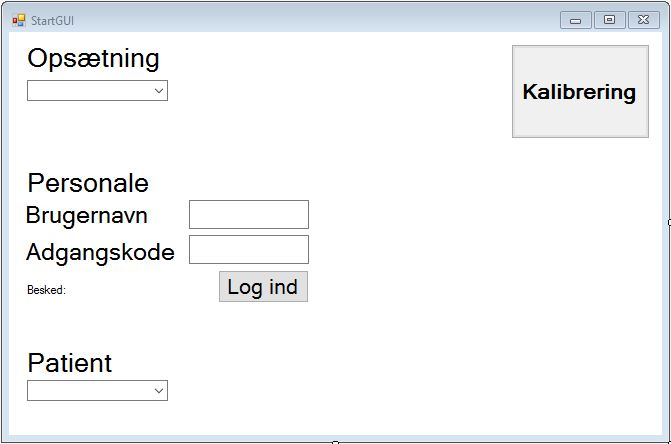
\includegraphics[width =0.4\textwidth , center]{billeder/skitseStart}
\caption{Skitse af startskærmen, som repræsenterer EPJ systemet}
\end{figure}
\begin{figure}[h!]
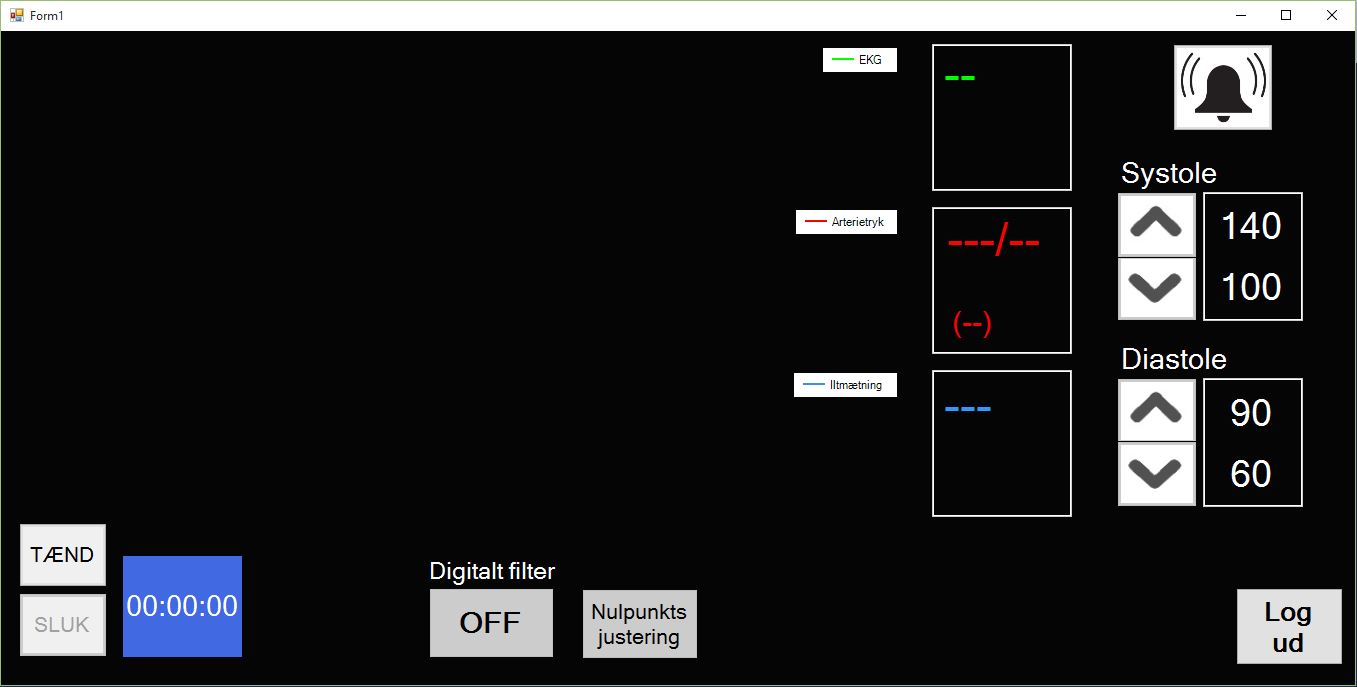
\includegraphics[width =1.0\textwidth , center]{billeder/skitseHoved}
\caption{Skitse af hovedskærmen, hvilken repræsenterer en blodtryksmålers brugergrænseflade}
\end{figure}
\end{enumerate}
\item \textbf{Reliability}
\begin{enumerate}
\item (\textbf{S}) INGEN RELIABILITY KRAV ENDNU
\end{enumerate}
\item \textbf{Performance}
\begin{enumerate}
\item (\textbf{S}) Tiden der går før måling af data påbegynder/vises i grafer må maksimalt være 2 sek.
\item (\textbf{S}) Tiden der går fra at data, herunder puls, diastolisk tryk, systolisk tryk og middeltryk, er analyseret til at data er gemt i EPJ database må være 2 sek. med en tolerance på +/-15\% 
\item (\textbf{S}) Ved justering af grænseværdi for systole og diastole ændres grænseværdien 1 mmHg op eller ned.                                                                                                                                                                                                                                                                                                                                                                                                                                                                                                                                                                                                                                                                                               
\end{enumerate}
\item \textbf{Supportability}
\begin{enumerate}
\item (\textbf{M}) Programmet skal skrives i Csharp kode
\item (\textbf{M}) Softwaren skal være opbygget efter trelagsmodellen (Data-View-Model)
\item (\textbf{S}) I softwaren benyttes Observer/Subject mønsteret.
\item (\textbf{S}) I softwaren benyttes PUSH mønsteret
\end{enumerate}
\item \textbf{+ Test conditions}
\begin{enumerate}
\item (\textbf{M}) Der skal være adgang til en computer med Windows 7, 8 eller 10 - computeren skal minimum have 4 GB RAM.
\item (\textbf{M}) Der skal være adgang til en computer hvor National Instruments er installeret.
\end{enumerate}
\end{enumerate}
\chapter{Arkitektur og design}
Følgende beskriver arkitekturen for systemet herunder både hardware og software. 
Systemarkitektur er udviklingsrammen for den videre udvikling af design og implementering. Der vil igennem dette afsnit startes med at se systemet overordnet og hvorefter der arbejdes ned gennem systemet i mindre brudstykker. Der benyttes diagrammer for at kunne specificere og klarlægge systemkravene. Disse diagrammer beskrives desuden i tekst. Igennem dette afsnit bliver designet af produktet dermed bestemt.
\section{Hardware design}
\subsection{Implementering}
\subsubsection{Block definition diagram}
På nedenstående figur bliver systemets hardware illustreret i et BDD. Heraf ses det at systemet har seks hardware blokke: Computer, transducer, NI-DAQ, lavpas filter, forstærker og en strømforsyning. Disse blokke udgør tilsammen blodtryksmålersystemet.
\begin{figure}[H]
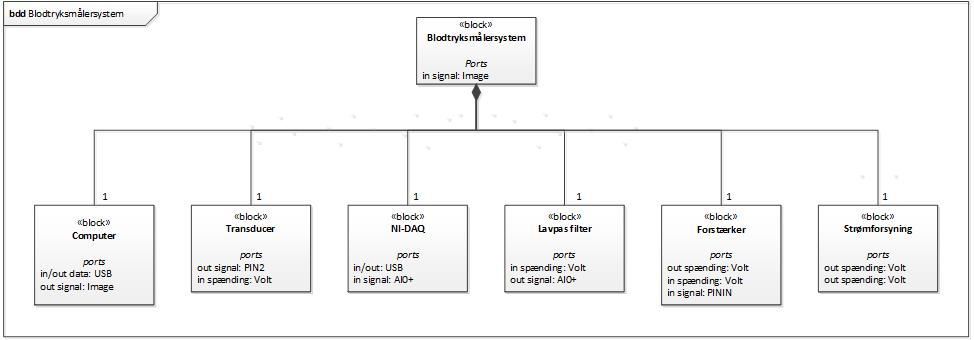
\includegraphics[width =1.0\textwidth , center]{billeder/BDD}
\caption{\textbf{Block definition diagram. Dette diagram viser hardware delene i systemet, samt sammenhængen mellem disse.}}
\end{figure}
\subsubsection{Internal block definition}
Ud fra BDD kan et IBD diagram udarbejdes. IBD diagrammet viser koblingen mellem blokkene:
\begin{itemize}
\item Strømforsyningen, denne er to 9V batterier som forsyner forstærkeren og transduceren med $\pm$ 9V
\item Transduceren omdanner tryksignalet fra kateteret til et strømsignal i ZZ mV tilbage til forstærkeren.
\item Forstærkeren forstærker signalet til lavpas filteret.
\item Lavpas filteret dæmper de høje frekvenser og sender signalet til NI-DAQ
\item NI-DAQs formål er, at omdanne signalet fra et analogt signal til et digitalt signal.
\item Computerens funktion er at få analyseret og vist blodtryksignalet på en brugergrænseflade, vha. Visual Studio. 
\end{itemize}
\begin{figure}[H]
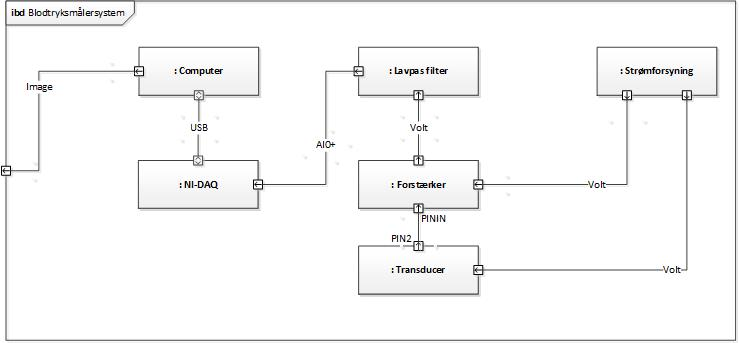
\includegraphics[width =1.0\textwidth , center]{billeder/IBD}
\caption{\textbf{Internal block diagram. Dette diagram viser signalerne imellem blokkene.}}
\end{figure}

\subsection{Modultest}
\section{Software design}
I dette afsnit beskrives softwaredesign på baggrund af systembeskrivelsen og kravspecifikationen. Denne beskrivelse opnås ved at der benyttes relevante diagrammer og modeller, hvilke kan bruges til at beskrive softwaren. Overvejelser og valg, der er blevet gjort, i forbindelse med design og implementering af softwaren, vil i dette afsnit blive præsenteret.
\subsection{Problemidentifikation}
\subsubsection{Domænemodel}
Først skal der klarlægges hvilke klasser som systemet skal bestå af, hvilket er det første skridt i processen. For at kunne identificere disse klasse udarbejdes en domænemodel, hvilken har sit udgangspunkt i Use cases. Det er i de konceptuelle klasser fra Use cases som indeholder den information som systemet skal holde styr på. Derfor findes de konceptuelle klasser i Use cases og disse indføres i domænemodellen som klasser. Domænemodellen opstilles derfor for at finde frem til hvad problemet er i softwaren i forhold til, hvad der skal holdes styr på.
\begin{figure}[H]
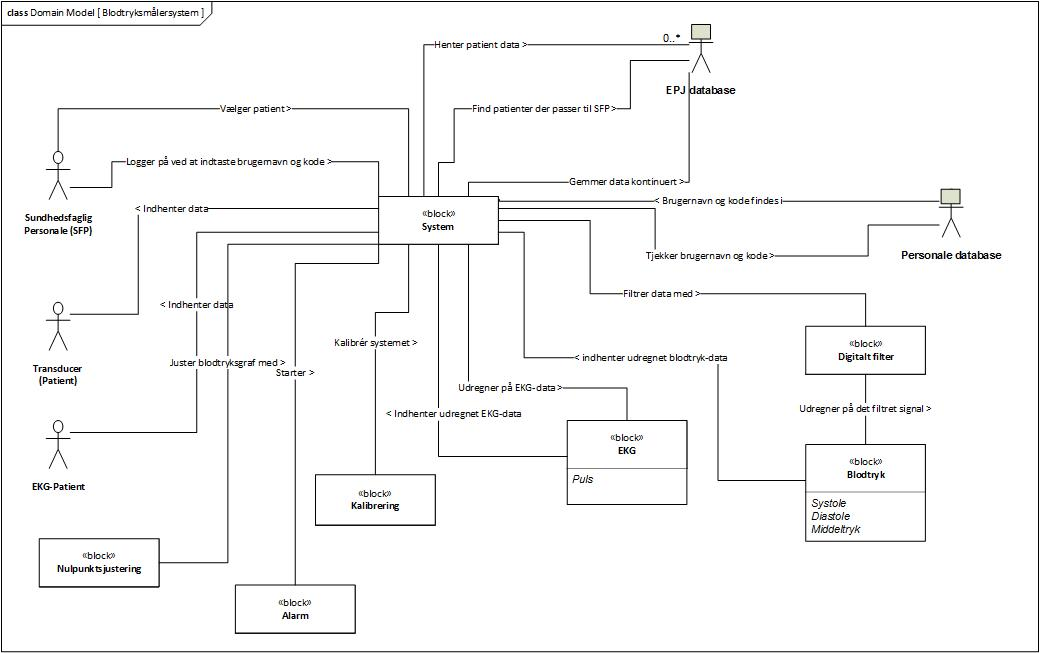
\includegraphics[width =1.0\textwidth , center]{billeder/DM}
\caption{\textbf{Domænemodel for blodtryksmålersystemet.}}
\end{figure}
Denne domænemodel viser det sundhedsfaglige personales interaktion med systemet, samt hvilke handlinger der startes af denne interaktion. Det sundhedsfaglige personale udfører en handling, der medfører, at en række processer igangsættes i systemet. Disse processer sørger at hente data fra transduceren og EKG patient, sørger for at starte beregningen af puls, systolisk, diastolisk og middeltryks værdierne og vise disse på brugergrænsefladen, samt sørger for at disse data bliver gemt i en database.
\newpage
\subsection{Klasseidentifikation}
\subsubsection{Applikationsmodel}
Ud fra domænemodellen kan en applikationsmodel opstilles. Denne model tager afsæt i domænemodellens klasser. Dette betyder derfor at denne model således også tager udgangspunkt i alle Use cases.\\
Modellen bruges til at bestemme de interagerende klasser i blodtryksmålersystemet.\\
\begin{figure}[H]
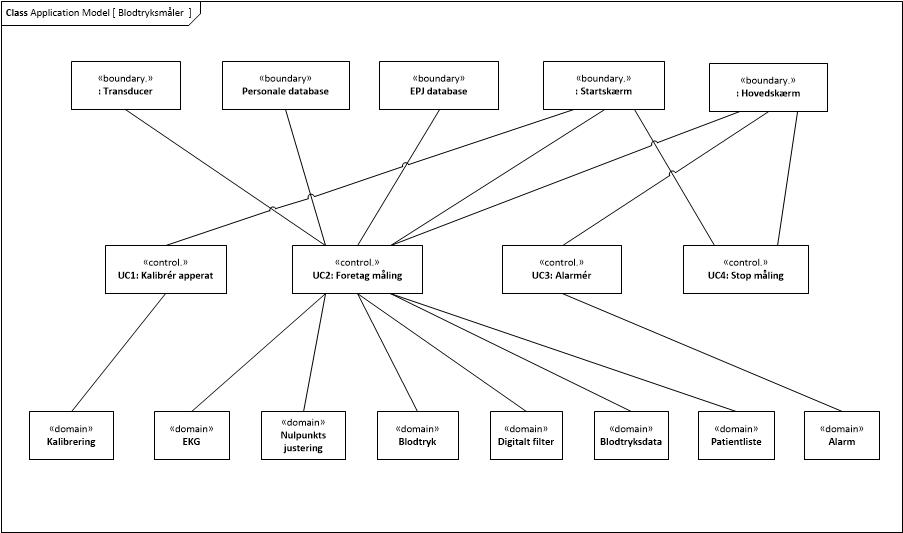
\includegraphics[width =1.0\textwidth , center]{billeder/appModel}
\caption{\textbf{Applikationsmodel for blodtryksmålersystemet.}}
\end{figure}
Ud fra denne model ses klasserne og databaserne der skal implementeres i softwaren, samt interaktionen mellem disse. Altså hvordan klasserne må tale sammen på kryds og tværs. Så idet at det vides at tre-lagsmodellen skal benyttes, kan disse klasser ligges ind i det tilhørende lag. Databaserne vil blive tilgået fra datalaget, domæneklasserne ligger i logiklaget og i præsentationslaget vil startskærmen og hovedskærmen ligge hvorfra de vil blive præsenteret for det sundhedsfaglige personale.
\subsection{Metodeidentifikation}
\subsubsection{Sekvensdiagrammer}
Nedenfor er vist sekvensdiagrammer for systemet. Der er lavet sekvens diagrammer for alle Use case. Vores Use cases er henholdsvis Use case 1: Kalibrér system, Use case 2: Foretag måling, Use case 3: Alarmér og Use case 4: Stop måling. Sekvens diagrammet er et interaktionsdiagram, som viser hvorledes processerne forløber i forhold til hinanden. Ud fra sekvensdiagrammerne kan det altså ses hvornår og hvordan de forskellige dele i systemet forløber og interagerer. \\
\begin{figure}[H]
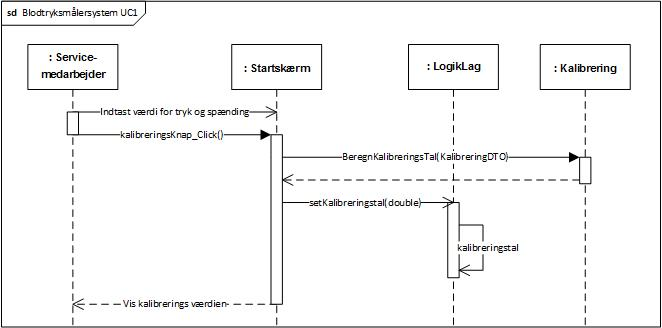
\includegraphics[width =1.0\textwidth , center]{billeder/sdUC1}
\caption{\textbf{Sekvensdiagram for blodtryksmålersystemet. Denne viser adfærden for Use case 1 }}
\end{figure}
I sekvens diagrammet for Use case 1 interagerer servicemedarbejder med blodtryksmålersystemet. Her er det servicemedarbejderen som starter kalibreringen og blodtryksmålersystemet som foretager kalibreringen igennem lagene og klassen Kalibring. Her ses det at servicemedarbejderen indtaster værdierne der aflæses, hvorefter der trykkes på knappen, hvorefter systemet foretager beregningen for kalibreringen.\\\\ 
\begin{figure}[H]
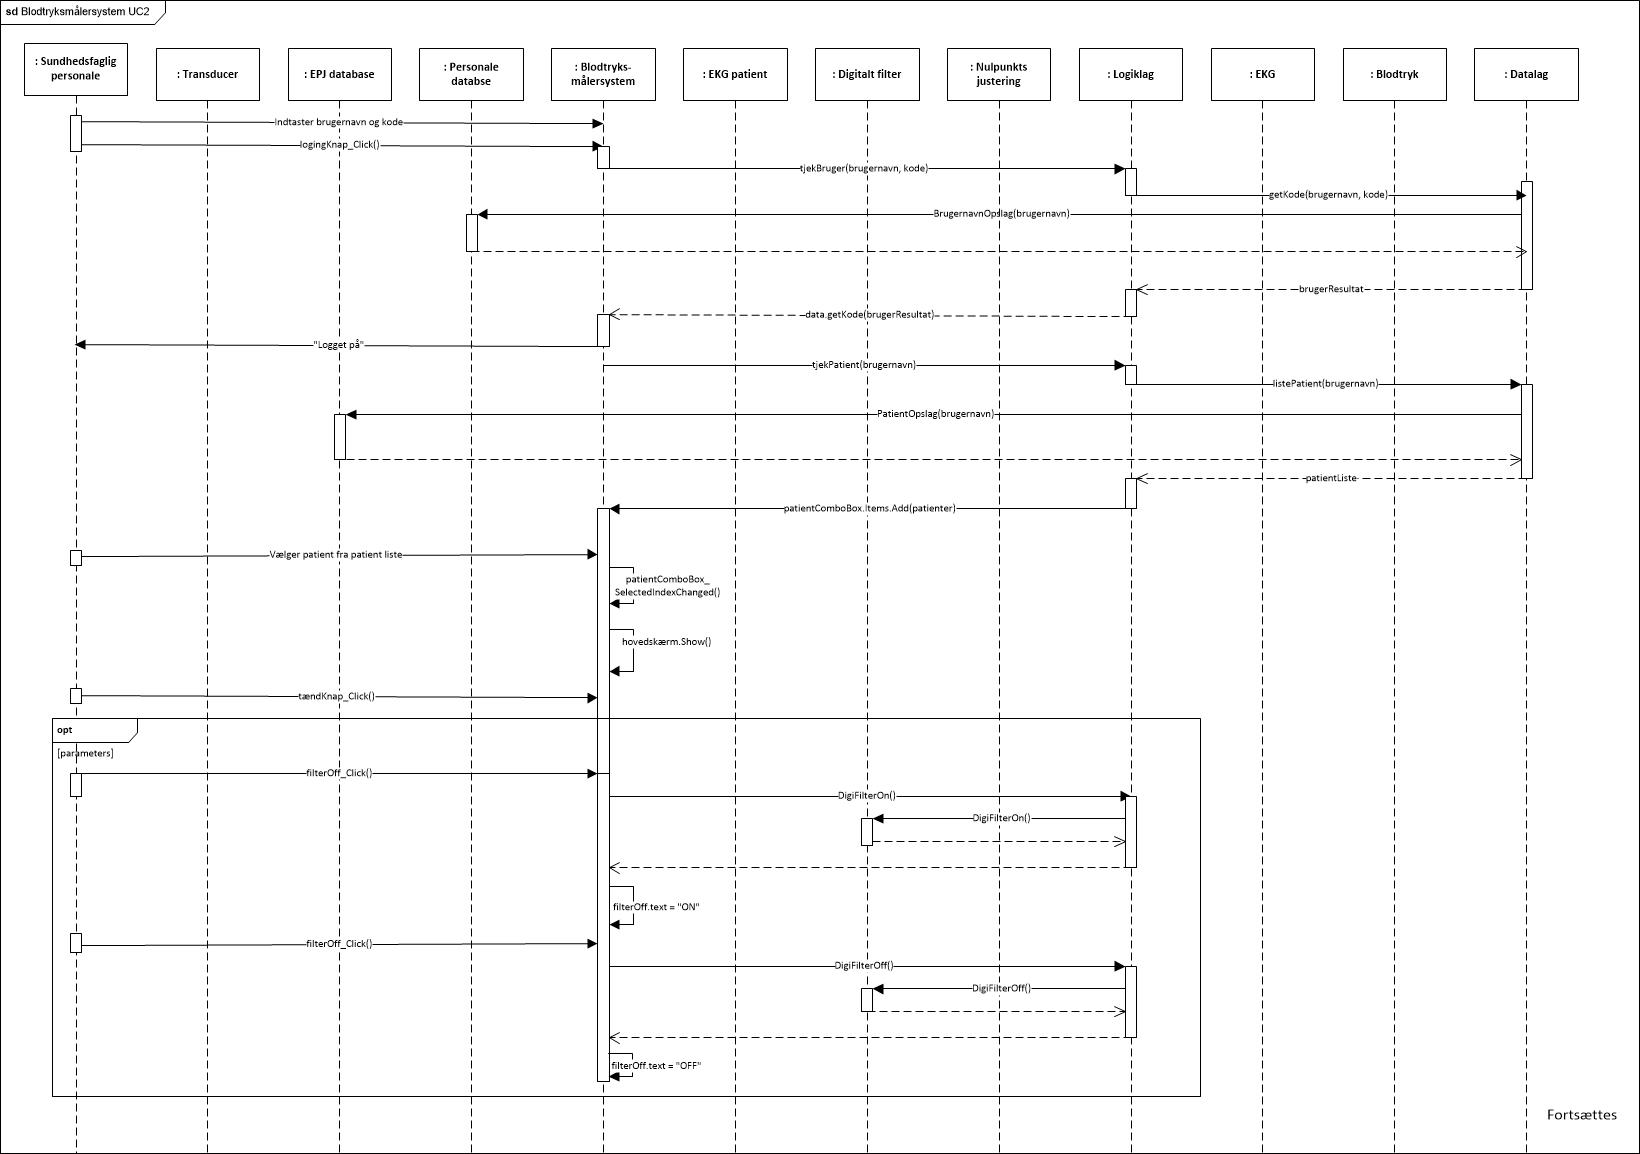
\includegraphics[width =1.0\textwidth , center]{billeder/sdUC2}
\caption{\textbf{Sekvensdiagram for blodtryksmålersystemet. Denne viser adfærden for Use case 2 del 1}}
\end{figure}
\begin{figure}[H]
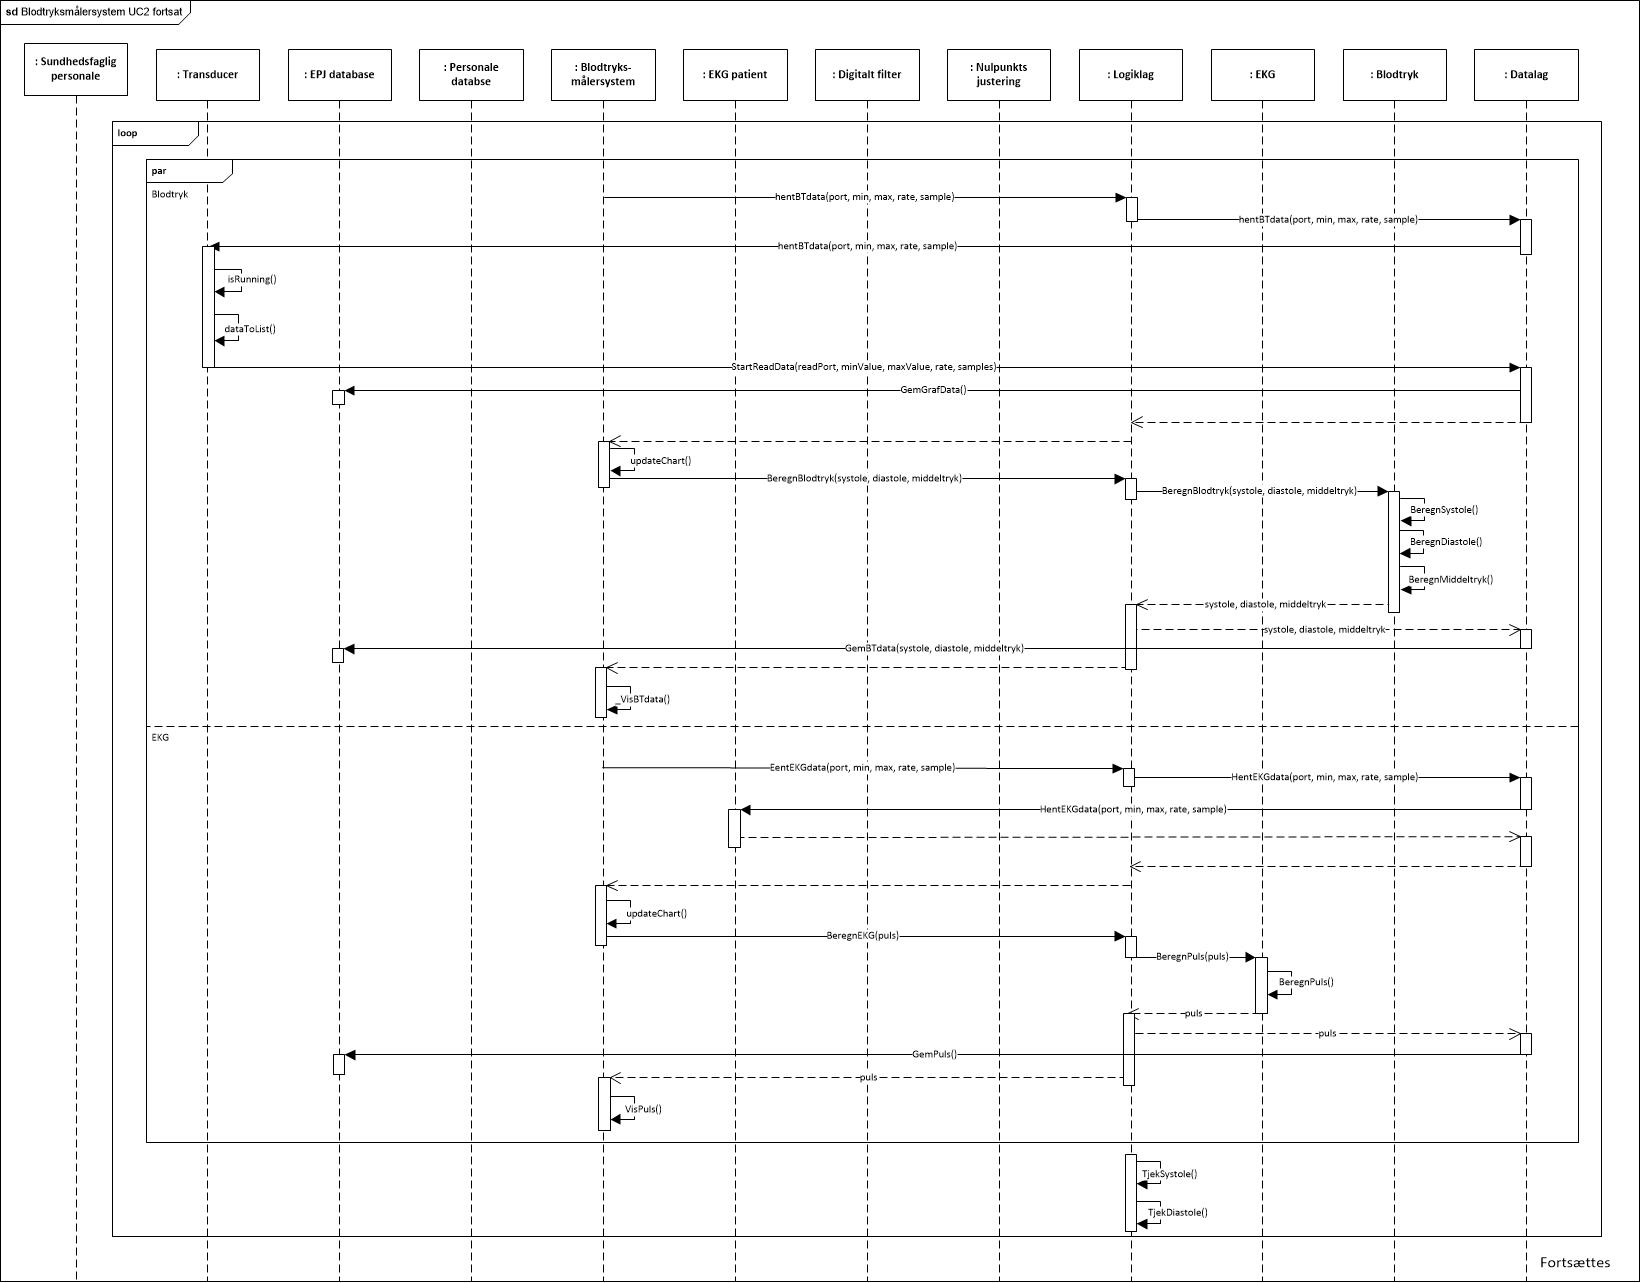
\includegraphics[width =1.0\textwidth , center]{billeder/sdUC2_2}
\caption{\textbf{Sekvensdiagram for blodtryksmålersystemet. Denne viser adfærden for Use case 2 del 2}}
\end{figure}
\begin{figure}[H]
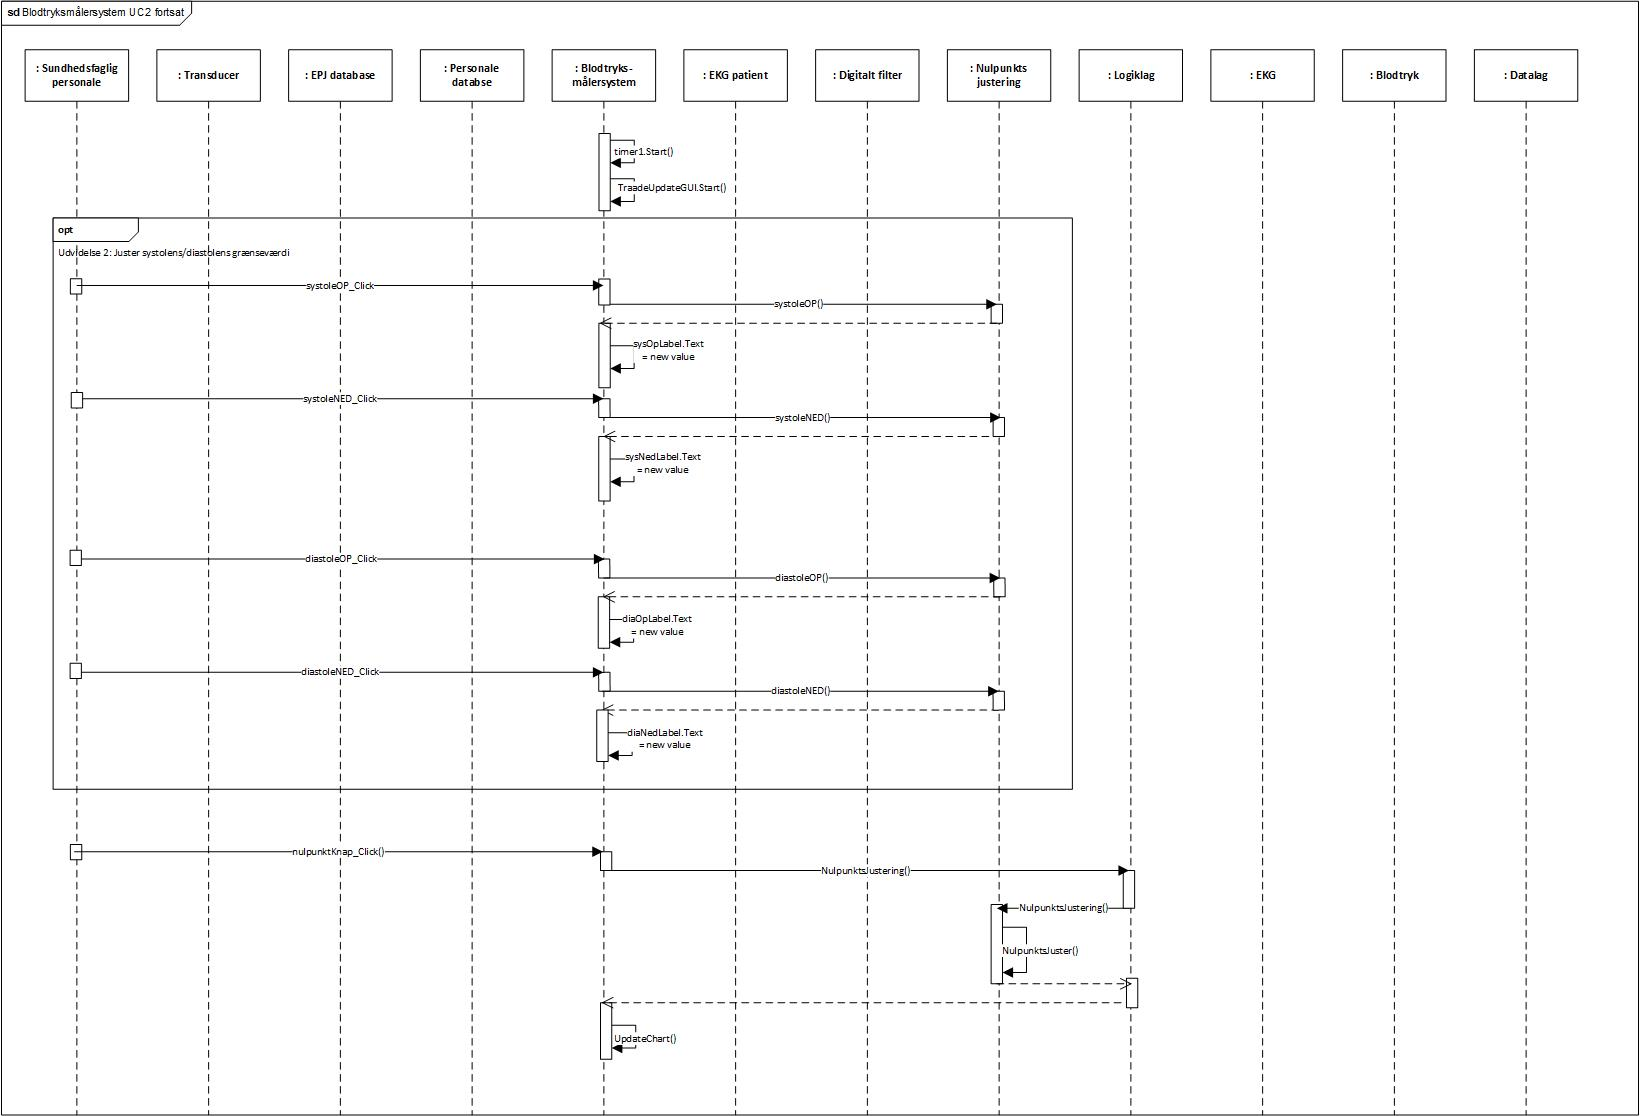
\includegraphics[width =1.0\textwidth , center]{billeder/sdUC2_3}
\caption{\textbf{Sekvensdiagram for blodtryksmålersystemet. Denne viser adfærden for Use case 2 del 3}}
\end{figure}
I sekvens diagrammet for Use case 2 ønsker det sundhedsfaglig personale at foretage måling, dette gøres ved at det sundhedsfaglig personale interagerer med blodtryksmålersystemet. For at målingen forløber, foregår den videre interaktion via blodtryksmålersystemet og de klasser, som indgår i Use casen. Transducer, EKG patient sender sine data til datalaget, EPJ database og Personale database får sine data fra datalaget. I dette sekvens diagram ses det sundhedsfaglige personales interaktion med blodtryksmålersystemet. Denne interaktion igangsætter processerne, som medfører at blodtryksmålingen forløber. Det ses også, at præsentationslaget, som er vores blodtryksmålersystem, kommunikerer med logiklaget og logiklaget kommunikerer med datalag, altså er trelagsmodellen opfyldt. \\\\
\begin{figure}[H]
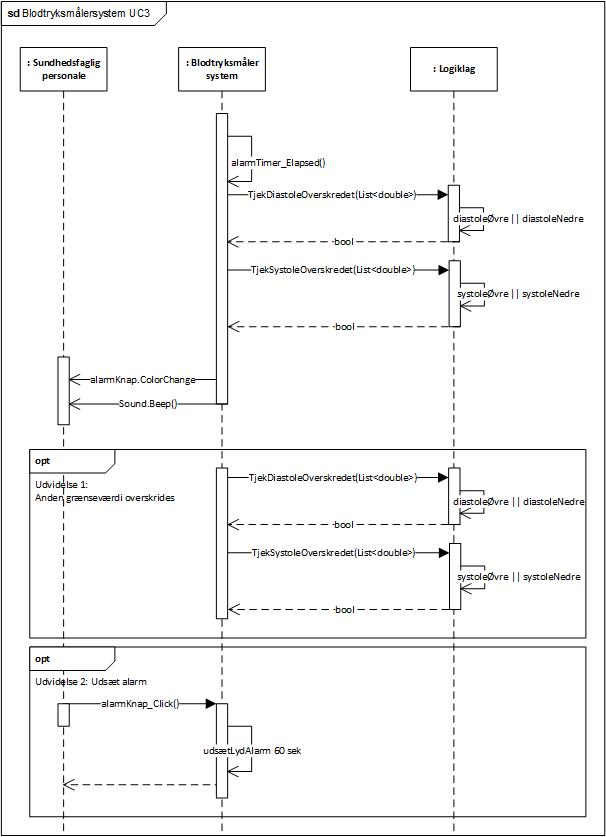
\includegraphics[width =1.0\textwidth , center]{billeder/sdUC3}
\caption{\textbf{Sekvensdiagram for blodtryksmålersystemet. Denne viser adfærden for Use case 3}}
\end{figure}
I dette sekvens diagram for Use case 3 tjekker logiklaget hvorvidt grænseværdierne for systole og diastole er overskredet. Hvis en grænseværdi overskrides starter alarmeringen. I denne Use case har det sundhedsfaglig personale mulighed for at udsætte alarmen, dette sker ved en interaktion mellem sundhedsfaglig personale og blodtryksmålersystemet.\\\\ 
\begin{figure}[H]
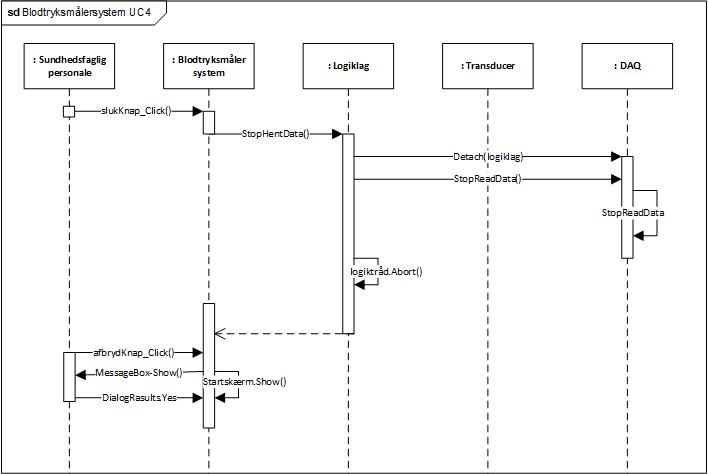
\includegraphics[width =1.0\textwidth , center]{billeder/sdUC4}
\caption{\textbf{Sekvensdiagram for blodtryksmålersystemet. Denne viser adfærden for Use case 4}}
\end{figure}
I sekvens diagrammet for Use case 4 ønsker sundhedsfaglig personale, at stoppe målingen. Dette gøres ved, at sundhedsfaglig personale interagerer med blodtryksmålersystemet i præsentationslaget. Denne interaktion medfører en videre kommunikation mellem logiklaget og datalaget, som medfører at data ikke længere hentes fra transduceren. Når blodtryksmålingen er afsluttet vises det som besked til det sundhedsfaglig personale. 

\subsection{Implementering}
Under implementeringen af produktet er der opstået nogle vanskeligheder, som der har skullet tages hensyn til. Der blev f.eks. i første omgang udarbejdet en idé om at have en brugergrænseflade, som startskærm, hvor det kunne vælges hvorpå målingen skulle foretages. På startskærmen skulle det desuden være muligt at kalibrere systemet og foretage nulpunkts justeringen. Stederne hvor målingerne skulle foretages blev identificeret til at skulle være 3 målesteder; hjertet, armen og benet. Efter stedet var valgt, hvor målingen skulle foretages, skulle man komme videre til en anden skærm, hvor selve målingen skulle foretages. Denne idé viste sig dog ikke at være brugbar i praksis, hvilket fik os til at gå væk fra denne. Grunden til at denne idé ikke ville kunne bruges i praksis, ved en invasiv blodtryksmåling, var at denne idé var tænkt som et produkt til måling på diabetes patienter, men ved denne patientgruppe er det ikke hensigtsmæssigt at lave hul i karrene på bl.a. benene, da blodtrykket her vil være lavt og helingen af det hul, der bliver lavet i benet, derfor ikke vil kunne foregå optimalt og der vil være risiko for infektioner. \\
\begin{figure}[H]
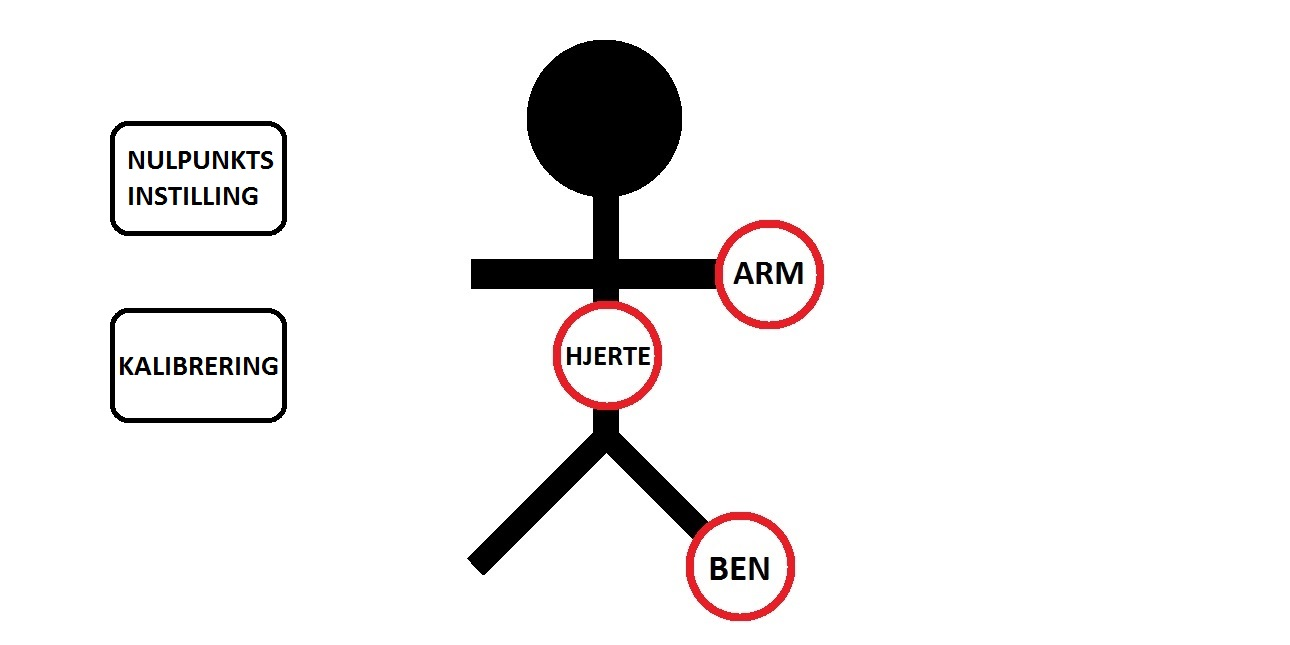
\includegraphics[width =0.5\textwidth , center]{billeder/SkitseStartGammel}
\caption{\textbf{Idé til projekt}}
\end{figure}
Herefter blev idéen ændret til et produkt, der ligner noget der fungerer i dagligdagen på hospitalerne. Denne idé blev udarbejdet efter et besøg på Herning Sygehus. Her blev det muligt at se hvordan en blodtryksmåler virker i virkeligheden, og dermed se hvordan disse blodtryksmålere benyttes.\\
Ved denne idé blev en startskærm, som skal simulere EPJ-systemet, udarbejdet. EPJ-systemet er der, hvor det sundhedsfaglige personale kan tilgå patientens data, og dermed evt. se hvilket behandling patienten har været igennem før. Startskærm der her er udarbejdet, er blot en prototype af dette og derfor er det kun den del hvor det sundhedsfaglige personale logger på, samt vælger patient, der er blevet implementeret. Dermed er det ikke muligt at tilgå tidligere behandlinger osv. som det er i virkeligheden. Det blev desuden klart at nulpunkts justeringen, hvilken der hertil var placeret på startskærmen, skulle flyttes ind på hovedskærmen, altså skærmen, hvor selve målingen foretages. Dette skulle den idet der skal være data for at nulpunkts justeringen kan foretages. Kalibreringen skal dog stadig foretages inden data sendes ind i systemet, og er dermed stadig placeret på startskærmen. Kalibreringen foretages med en væskesøjle, hvor der er tre punkter, som fører til at en spænding kan aflæses. Ud fra det tryk der leveres af væskesøjlen samt den målte spænding, kan en hældningskoefficient bestemmes, hvilken systemet skal gemme til at regne på alle data.\\
Ud fra alle disse faktorer kan grundstrukturen, til hvordan startskærmen og hovedskærmen skal se ud, dannes.
\begin{figure}[H]
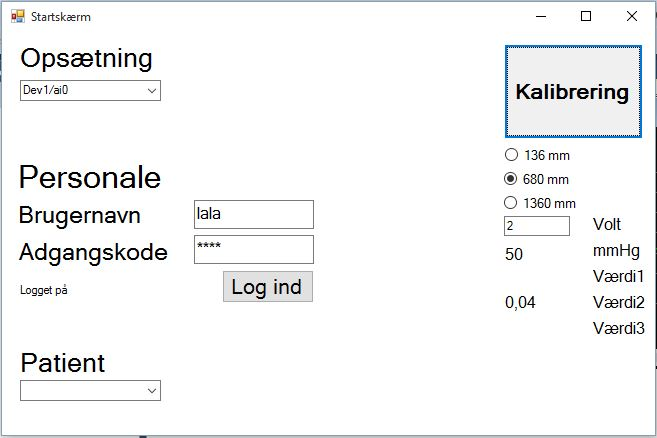
\includegraphics[width =0.5\textwidth , center]{billeder/SkitseStartNy}
\caption{\textbf{Startskærmen, hvilken fungerer som EPJ-systemet}}
\end{figure}
\begin{figure}[H]
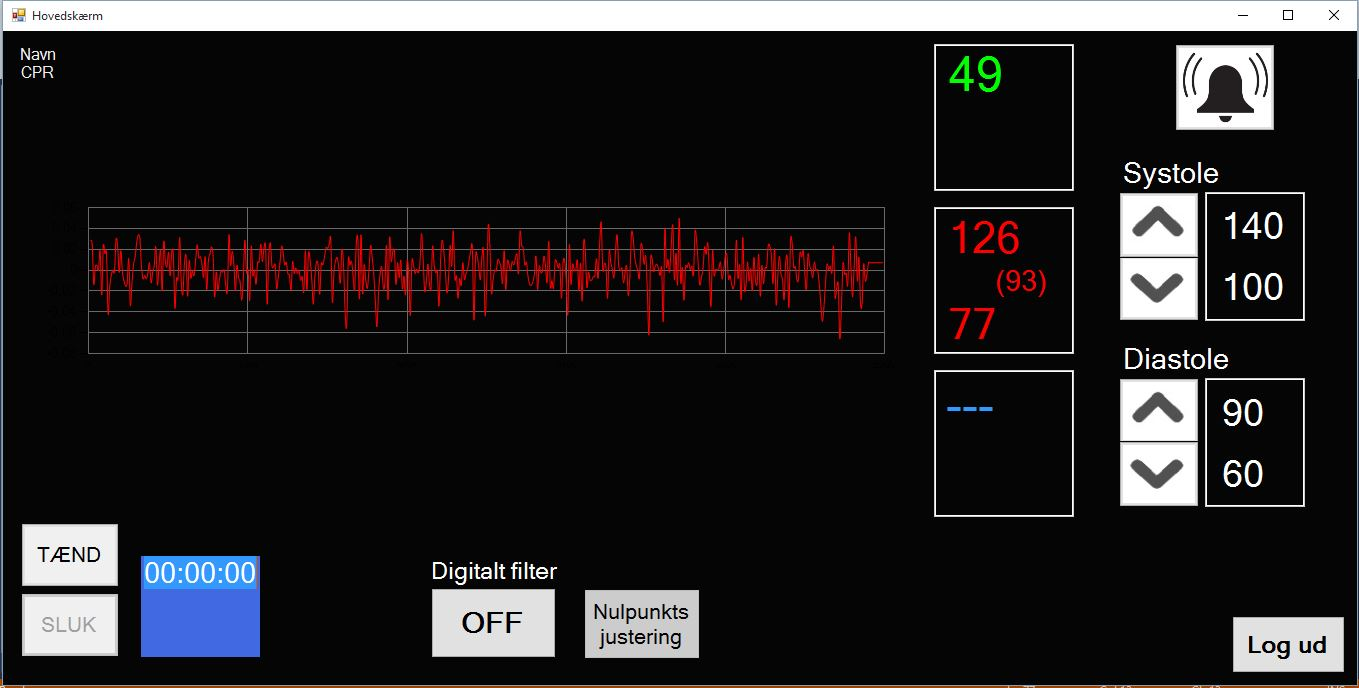
\includegraphics[width =0.8\textwidth , center]{billeder/SkitseHovedNy}
\caption{\textbf{Hovedskærmen, hvilken fungerer som blodtryksmålerens grænseflade}}
\end{figure}

Baggrund for:
Nulpunktsjustering 
Kalibrering 
Digitalt filter
Beregning af Systole og diastole - middeltryk

Acceptering af tidspres: EKG: kan ikke nås



\subsection{Unittest}
\section{Integrationstest}


\chapter{Accepttest}
\section{Indledning}
Accepttestene skal vise om kravene der er opstillet for blodtryksmålersystemet i kravspecifikationen lever op til de standarder der er sat op for at produktet aktivt kan indgå i en hverdag på sygehusene.\\
Accepttestene er er opfølgning af kravspecifikationen, hvilket sikre at alle krav er overholdt og dermed opnået.\\\\
Når der i feltet Godkendt er skrevet initialer for den der har udført testen, samt datoen for testens udførelse, betyder det at testen er godkendt.  \\

\section{Accepttest for funktionelle krav}
\subsection{Opstilling}
Billede indsættes - haves ikke endnu

\begin{table}[H]
\caption{Accepttest for Use case 1}\label{tab:tabel8}
\begin{tabular}{|>{\raggedright\arraybackslash}p{2.5cm}| >{\raggedright\arraybackslash}p{2.9cm} | >{\raggedright\arraybackslash}p{2.9cm} | >{\raggedright\arraybackslash}p{2.9cm} | >{\raggedright\arraybackslash}p{2.8cm} |}
   \hline
   \textbf{Use case 1: Kalibrer apparat} &\textbf{Test}& \textbf{Prækondition} & \textbf{Forventet resultat} & \textbf{Godkendt/ kommentar}\\ \hline
   Normalforløb:& Vælg hvilken af de tre punkter kalibreringen udføreres på. & Blodtryksmålersystemet er tændt og tilsluttet, og tilsluttet kalibreringsudstyret (Analog Discovery og Waveforms). & Værdien for tryk i mmHg for målepunktet vises på GUI & \\hline
   &Indtast den aflæste værdi fra Waveforms og tryk på "Kalibrering" & Blodtryksmålersystemet er tændt og tilsluttet, og tilsluttet kalibreringsudstyret (Analog Discovery og Waveforms) og målepunkt valgt. & Systemet er kalibreret resultatet af beregningen vises på startskærmen & IKKE TESTBAR\\\hline
\end{tabular}
\end{table}



\begin{table}[H]
\caption{Accepttest for Use case 2}\label{tab:tabel8}
\begin{tabular}{|>{\raggedright\arraybackslash}p{2.5cm}| >{\raggedright\arraybackslash}p{2.9cm} | >{\raggedright\arraybackslash}p{2.9cm} | >{\raggedright\arraybackslash}p{2.9cm} | >{\raggedright\arraybackslash}p{2.8cm} |}
   \hline
   \textbf{Use case 2: Foretag måling} &\textbf{Test}& \textbf{Prækondition} & \textbf{Forventet resultat} & \textbf{Godkendt/ kommentar}\\ \hline
   Normalforløb:& Indtast brugernavn "anpe" og kode "1234" & Port valgt. VPN, Personale database og EPJ database er tilsluttet korrekt & Korrekt indtastning fuldendt & \\\hline
   &Tryk "Login" & Port valgt. VPN, Personale database og EPJ database er tilsluttet korrekt & Besked: "Logget på" og den sundhedsfaglige er dermed logget på &\\\hline
   &Tryk på patient dropdown på startskærm & En sundhedsfaglig er logget på & Liste med patienter kommer frem  & \\\hline
   & Vælg patienten "Arne Jensen" & Den sundhedsfaglige er logget på & Nyt vindue kommer frem: Hovedskærmen &\\\hline
   & Tryk på "Tænd"& Patient valgt og blodtryksmålersystemet (transduceren) er tilsluttet & Systemet indhenter data fra transduceren og starter timer på hovedskærm. EKG og arterietryk præsenteres kontinuert på hver sin graf. Puls, systole, diastole og middeltryk vises som talværdier på hovedskærmen. Data gemmes automatisk kontinuert i EPJ database & \\\hline
   & Tryk på "Nulpunkts justering" & Signalet er startet og kører & Systemet starter nulpunkts justeringen. Systemet tilpasser grafen. &\\\hline
\end{tabular}
\end{table}



\begin{table}[H]
\caption{Accepttest for Use case 2}\label{tab:tabel8}
\begin{tabular}{|>{\raggedright\arraybackslash}p{2.5cm}| >{\raggedright\arraybackslash}p{2.9cm} | >{\raggedright\arraybackslash}p{2.9cm} | >{\raggedright\arraybackslash}p{2.9cm} | >{\raggedright\arraybackslash}p{2.8cm} |}
   \hline
   \textbf{Use case 2: Foretag måling} &\textbf{Test}& \textbf{Prækondition} & \textbf{Forventet resultat} & \textbf{Godkendt/ kommentar}\\ \hline
   Undtagelse 1: Brugernavn og/eller kode indtastet forkert & Indtast brugernavn "efgh" og kode "1234"& Port valgt. VPN, Personale database og EPJ database er tilsluttet korrekt & Forkert kombinition indtastet &  \\\hline
   &Tryk "Login" & Port valgt. VPN, Personale database og EPJ database er tilsluttet korrekt. & Besked: "Brugernavn og/eller kode indtastet forkert" &\\\hline
\end{tabular}
\end{table}



\begin{table}[H]
\caption{Accepttest for Use case 2}\label{tab:tabel8}
\begin{tabular}{|>{\raggedright\arraybackslash}p{2.5cm}| >{\raggedright\arraybackslash}p{2.9cm} | >{\raggedright\arraybackslash}p{2.9cm} | >{\raggedright\arraybackslash}p{2.9cm} | >{\raggedright\arraybackslash}p{2.8cm} |}
   \hline
   \textbf{Use case 2: Foretag måling} &\textbf{Test}& \textbf{Prækondition} & \textbf{Forventet resultat} & \textbf{Godkendt/ kommentar}\\ \hline
   Udvidelse 1: Slå digitalt filter til/fra:& Tryk på "Digitalt filter OFF" & Signalet er startet & Systemet slår det digitale filter fra. De to signaler (XX Hz og YY Hz) er indsendt og knappen ændrer navn &\\\hline
   &Tryk på "Digitalt filter ON" & Signalet er startet & Systemet slår det digitale filter til. Den ene (XX Hz) af de indsendt signaler er blevet fjernet og knappen ændre navn. &\\\hline
\end{tabular}
\end{table}


\begin{table}[H]
\caption{Accepttest for Use case 2}\label{tab:tabel8}
\begin{tabular}{|>{\raggedright\arraybackslash}p{2.5cm}| >{\raggedright\arraybackslash}p{2.9cm} | >{\raggedright\arraybackslash}p{2.9cm} | >{\raggedright\arraybackslash}p{2.9cm} | >{\raggedright\arraybackslash}p{2.8cm} |}
   \hline
   \textbf{Use case 2: Foretag måling } &\textbf{Test}& \textbf{Prækondition} & \textbf{Forventet resultat} & \textbf{Godkendt/ kommentar}\\ \hline
   Udvidelse 2: Juster systolens/diastolens grænseværdi& Tryk på "Systole op"/"Diastole op"& Signalet er startet & Grænseværdien ændres 1 mmHg op og intervallet vises på hovedskærmen &\\\hline
   &Tryk på "Systole ned"/"Diastole ned" & Signalet er startet & Grænseværdien ændres 1 mmHg ned og intervallet vises på hovedskærmen & \\\hline
\end{tabular}
\end{table}



\begin{table}[H]
\caption{Accepttest for Use case 3}\label{tab:tabel8}
\begin{tabular}{|>{\raggedright\arraybackslash}p{2.5cm}| >{\raggedright\arraybackslash}p{2.9cm} | >{\raggedright\arraybackslash}p{2.9cm} | >{\raggedright\arraybackslash}p{2.9cm} | >{\raggedright\arraybackslash}p{2.8cm} |}
   \hline
   \textbf{Use case 3: Alarmér } &\textbf{Test}& \textbf{Prækondition} & \textbf{Forventet resultat} & \textbf{Godkendt/ kommentar}\\ \hline
   Normalforløb:& Grænseværdi overskrides& Signalet er startet & Alarm starter med lyd og tallet, hvis grænseværdi er overskredet, ændrer farve til hvid &\\\hline
   & Grænseværdien er ikke overskredet mere & Alarmen igangsat & Alarm lyden stopper og tallet skifter farve tilbage til rød. & \\\hline
\end{tabular}
\end{table}



\begin{table}[H]
\caption{Accepttest for Use case 3}\label{tab:tabel8}
\begin{tabular}{|>{\raggedright\arraybackslash}p{2.5cm}| >{\raggedright\arraybackslash}p{2.9cm} | >{\raggedright\arraybackslash}p{2.9cm} | >{\raggedright\arraybackslash}p{2.9cm} | >{\raggedright\arraybackslash}p{2.8cm} |}
   \hline
   \textbf{Use case 3: Alarmér } &\textbf{Test}& \textbf{Prækondition} & \textbf{Forventet resultat} & \textbf{Godkendt/ kommentar}\\ \hline
   Udvidelse 1: Anden grænseværdi overskrides & Endnu en grænseværdi overskrides & Signalet er er startet og en alarm er startet & Lyd fra første alarm fortsætter og det nye tallet som har overskredet grænseværdien skifter ligeledes farve til hvid &\\\hline
\end{tabular}
\end{table}



\begin{table}[H]
\caption{Accepttest for Use case 3}\label{tab:tabel8}
\begin{tabular}{|>{\raggedright\arraybackslash}p{2.5cm}| >{\raggedright\arraybackslash}p{2.9cm} | >{\raggedright\arraybackslash}p{2.9cm} | >{\raggedright\arraybackslash}p{2.9cm} | >{\raggedright\arraybackslash}p{2.8cm} |}
   \hline
   \textbf{Use case 3: Alarmér } &\textbf{Test}& \textbf{Prækondition} & \textbf{Forventet resultat} & \textbf{Godkendt/ kommentar}\\ \hline
   Udvidelse 2: Udsæt alarm & Tryk på "Udsæt alarm" & Alarmering er startet & Systemet stopper alarmens lyd i et minut, tallet er forsat skiftet til farven hvid &\\\hline
\end{tabular}
\end{table}




\begin{table}[H]
\caption{Accepttest for Use case 4}\label{tab:tabel8}
\begin{tabular}{|>{\raggedright\arraybackslash}p{2.5cm}| >{\raggedright\arraybackslash}p{2.9cm} | >{\raggedright\arraybackslash}p{2.9cm} | >{\raggedright\arraybackslash}p{2.9cm} | >{\raggedright\arraybackslash}p{2.8cm} |}
   \hline
   \textbf{Use case 4: Stop måling } &\textbf{Test}& \textbf{Prækondition} & \textbf{Forventet resultat} & \textbf{Godkendt/ kommentar}\\ \hline
   Normalforløb:& Tryk på "Sluk" & Målingen er foretaget & Målingen, signalet og timer på hovedskærmen stopper &\\\hline
   & Tryk på "Log ud" & Signalet er stoppet & Pop-up vindue kommer op: "Er du sikker?" &\\\hline
   &Tryk "Ja"&Signalet og målingen er stoppet& Startskærmen kommer frem og ny måling kan foretages &\\\hline
\end{tabular}
\end{table}


\begin{table}[H]
\caption{Accepttest for Use case 4}\label{tab:tabel8}
\begin{tabular}{|>{\raggedright\arraybackslash}p{2.5cm}| >{\raggedright\arraybackslash}p{2.9cm} | >{\raggedright\arraybackslash}p{2.9cm} | >{\raggedright\arraybackslash}p{2.9cm} | >{\raggedright\arraybackslash}p{2.8cm} |}
   \hline
   \textbf{Use case 4: Stop måling } &\textbf{Test}& \textbf{Prækondition} & \textbf{Forventet resultat} & \textbf{Godkendt/ kommentar}\\ \hline
Undtagelse 1: Tryk på "Nej" &Tryk "Nej" & Signalet og målingen er stoppet & Kommer tilbage til hovedskærmen &\\\hline
\end{tabular}
\end{table}


\newpage

\newpage

\newpage

\section{Accepttest for ikke-funktionelle krav}

\begin{longtable}{|>{\raggedright\arraybackslash}p{1.1cm}| >{\raggedright\arraybackslash}p{2.7cm} | >{\raggedright\arraybackslash}p{2.7cm} | >{\raggedright\arraybackslash}p{2.7cm} | >{\raggedright\arraybackslash}p{2.2cm} |>{\raggedright\arraybackslash}p{2.2cm}|}
   \caption{Accepttest for ikke-funktionelle krav}\label{tab:label13}
\\ \hline   
\textbf{Krav nr.}&\textbf{Krav} &\textbf{Test}& \textbf{Forventet resultat} & \textbf{Resultat} & \textbf{Godkendt/ kommentar}\\ \hline
  1.1 & Programmet skal have et digitalt filter til udglatning af blodtrykssignal & Send to frekvenser ind (XX Hz og ZZ Hz) & Den ene (XX Hz) af de indsendte frekvenser er blevet fjernet & & \\\hline
  1.2 & Programmet skal give alarm når grænseværdier overskrides med lyd og hvor den overskredede grænse værdi skifter farve til hvid på skærmen. & Overskrid en grænseværdi og tjek alarmering & Alarmen starter& & \\\hline
  1.3 & Programmet skal kunne gemme blodtrykssignalet i en database & Indsend signal og gå ind i databasen og se værdier & Der ligger værdier i databasen & & \\\hline\hline
  2.1 & Programmet skal have to window form: startskærm, der fungerer som EPJ systemet, og hovedskærm, som fungerer som selve blodtryksmåleren & Start program og tjek dette & Der er to window forms & & \\\hline
  2.2 & Programmet skal have en "Login" knap på startskærmen & Start program og tjek startskærm & Startskærmen har en "Login" knap & & \\\hline
  2.3 & Programmet skal have en "Kalibrering" knap på startskærmen & Start program og tjek startskærm & Startskærmen har en "Kalibrering" knap & & \\\hline
  2.4 &Sundhedsfaglig personale skal kunne ændre "device/enhedsnavn" i dropdown på startskærm & Start program og tjek startskærm & Der er en opsætnings dropdown på startskærmen, hvor device/enhedsnavn kan ændres. & & \\\hline
  2.5 & Programmet skal indeholde en dropdown, hvor patienten kan vælges på startskærmen & Start program, log på og tjek startskærm & Startskærmen har en dropdown med patienter & & \\\hline
  2.6 & Programmet skal have en "Nulpunkts indstilling" knap på hovedskærmen & Start program og tjek hovedskærm & Der er en "Nulpunkts indstilling" knap på hovedskærmen & & \\\hline
  2.7 & Programmet skal have en knap, til at slå det digitale filter fra og til, på hovedskærmen & Start program og tjek hovedskærm & Der er en "Digital filter" knap på hovedskærmen & & \\\hline
  2.8 & Programmet skal have knapper, til at justere systolisk og diastolisk grænseværdiintervaller op og ned, på hovedskærmen & Start program og tjek hovedskærm & Der er ialt fire knapper, som justerer grænseværdierne på hovedskærmen & & \\\hline
  2.9 & Programmet skal have en "Udsæt alarm" knap på hovedskærmen & Start program og tjek hovedskærm & Der er en "Udsæt alarm" på hovedskærmen & & \\\hline
  2.10 & Programmet skal have en "Tænd" knap på hovedskærmen & Start program og tjek hovedskærm & Hovedskærmen har en "Tænd" kanp& & \\\hline
  2.11 & Programmet skal have en "Sluk" knap på hovedskærmen & Tjek hovedskærm & Hovedskærmen har en "Sluk" knap & & \\\hline
  2.12 & Programmet skal have en "Log ud" knap på hovedskærmen & Start program og tjek hovedskærm & Der er en "Log ud" knap på hovedskærmen & & \\\hline
  2.13 & Teksten på startskærmen skal kunne aflæs fra 2 meters afstand med en synsstyrke i intervallet +/-1 & 10 personer med synsstyrke i intervallet +/-1 skal teste startskærmen  & Alle 10 personer kan læse teksten tydeligt & & \\\hline
  2.14 & Teksten og graferne på hovedskærmen skal kunne læses fra 2 meters afstand ved synsstyrke i intervellet på +/-1 & 10 personer med synsstyrke i intervallet +/-1 skal teste hovedskærmen & Alle 10 personer kan læse grafer og teksten på hovedskærmen & & \\\hline
 2.15 & Programmet skal præsentere arterietryk kontinuert, herudover vise systolisk værdi, diastolisk værdi og middeltryk som talværdier. & Start program og start målingen & Grafen vises kontinuert og talværdierne vises på hovedskærmen. & & \\\hline
  2.16 & Programmet skal præsentere EKG og puls & Start program og start målingen. & EKG vises kontinuert og pulsen vises som talværdi på hovedskærmen. & & \\hline
  2.17 & Programmet skal præsentere iltmætning som graf og talværdi. & Start program og start måling & Iltmætningens grafen vises kontinuert og iltmætning vises som talværdi på hovedskærm. & IKKE IMPLEMENTERET & \\\hline
  2.18 & Programmet skal præsentere grafer efter standard & Start program og tjek farver & EKG vises i lysegrøn, arterietryk vises i rød og iltmætning vises i lyseblå & & \\\hline
  2.19 & Programmet skal præsentere data i tal efter standard & Start program og tjek at talværdiernes farve er efter standard & Pulsværdien vises i lysegrøn, systolisk værdi, diastolisk værdi og middeltryk vises i rød og iltmætning vises i lyseblå.& & \\\hline\hline
  3.1 & Ingen krav endnu & & & & \\\hline\hline
  4.1 & Tiden der går før målingen af data påbegynder/vises i grafer må maksimalt være 2.0 sek. & Stopur igangsættes samtidig med at signalet tændes & Stopuret viser 2 sek. eller mindre & & \\\hline
  4.2 & Tiden der går fra at data er analyseret til at data er gemt i database må være 2.0 sek. med en tolerance på +/- 15\% & - & - & & \\\hline\hline
  5.1 & Programmet skrives i Csharp kode. & Tjek programmet & Programmet er skrevet i Csharp & & \\\hline
  5.2 & Softwaren skal være opbygget efter trelagsmodellen & Se programopbygningen & Softwaren er opbygget efter trelagsmodellen & & \\\hline
  5.3 & I softwaren benyttes Observer/Subject mønsteret & Tjek programmet og tjek observer/subject klasser & Observer og subject klasser/mønsteret benyttes & & \\\hline
  5.4 & I softwaren benyttes PUSH mønsteret & Tjek programmet & Det ses at programmet er opbygget efter PUSH mønsteret. & &  \\\hline \hline
  6.1 & Der skal være adgang til en computer med Windows 7, 8 eller 10 - computeren skal minimum have 4 GB RAM & & & & \\\hline
  6.2 & Der skal være adgang til en computer hvor National Instruments er installeret & & & & \\\hline
\end{longtable}

\section{Godkendelses formular}
\begin{table}[h!]
\label{tab:tabel14}
\begin{tabular}{| l | >{\raggedright\arraybackslash}p{12cm} |}
   \hline
   \textbf{Dato for test} &\\ \hline
   \textbf{Godkendes af:} & \\ \hline
\end{tabular}
\end{table}
\textbf{Ved underskrivelse af dette dokument godkendes den kørte accepttest}
\newline
\textbf{Sted og dato:}\\
\\
\\
\begin{table}
[h!]
\begin{tabular}{ l lllllllll l}
--------------------------------------&&&&&&&&&&--------------------------------------\\ 
Kundens underskrift &&&&&&&&&&Leverandørens underskrift\\
\end{tabular}
\end{table}

\chapter{Referencer}
\subsubsection{Bøger}
\subsubsection{Internetsider}
\subsubsection{Dokumenter}
